
\documentclass[]{emulateapj}
\usepackage{amsmath}
\begin{document}
\author{Draft}



\section{HST astrometry}
We adopt the VLA 5\,GHz map as the reference coordinate frame and shift the
coordinate frame in the optical image to this one to align the emission.

Employed local phase calibrator, with positions known to $\sim$1 mas, estimate
the absolute alignment of the 5 GHz and CO(J=2-1) coordinate frames should
be better than 0.1", leaving aside uncertainties relating to SNR and beam size.

The astrometry of the HST images was firstly calibrated against a wider-field
optical image of the cluster which had in turn been aligned onto the FK5
coordinate system to an rms precision of ~0.2".

%The align the IRAM data (2-mm continuum and CO(J=2-1)) with the VLA 5-GHz
%continuum emission, we shifted the former to the east by BLAH" in R.A., which is
%consistent with the claimed astrometric precision of the PdBI images.

To align the optical/NIR data with the VLA 5-GHz continuum emission, we
shifted the former in Dec. by +BLAH".



\section{CO($J$ = 3 $\rightarrow$ 2) line emission}

Analysis using both set 2 and set 3 observations. 

natural weighting beam size:  3.19 x 1.86 PA: 8 deg
channel width = 2x17.935 = 35.87 km/s
rms = 1.32997E-02 Jy/B/channel

 Integrated line flux = 37.509 Jy km/s over chan=[49,70] (FWZI)
%- ! Parameters and Errors:
%- ! MFIT%PAR[01]  
%- ! MFIT%PAR[02]  
%- ! MFIT%PAR[03]  
%- ! MFIT%PAR[04]  
%- velocity range [,] km/s

We have detected unresolved CO($J$ = 3 $\rightarrow$ 2) line emission toward
SMM J0939+8315 at peak flux at blah $\sigma$ signifcance of $ \sigma$ = 13.2997

mJy beam$^{-1}$.

We detect unresolved CO($J$ = 3 $\rightarrow$ 2) line emission toward the
background galaxies in RXJ1131-1231. 
We extract the spectrum and fit a single-component Gaussian as shown in Figure
\ref{fig:}
yielding peak flux density of BLAH $\pm$ BLAH mJy, the FWHM of the Gaussian fit
is BLAH $\pm$ BLAH km s$^{-1}$. 

\begin{figure}[tbph]
\centering
\includegraphics[width=0.5\textwidth]{../Figures/co32_spec_bin2.eps}	  
\caption{
CO32 line spectrum
 \label{fig:}}
\end{figure}


We made a 1.4mm continuum map using line-free channels, $\sigma$ = 8.30807E-04
Jy/B

At spatial position of CO emission, No significant continuum emission was
detected from the line-free region down to a 3$\sigma$ limit of blah mJy
(burried in noise - 
2.2 $\pm$ 3.0 mJy). Hence, we place a 3$\sigma$ upper limit of BLAH. 


%%%%%%%%%%%%%%%%%%%%%%%%%%%%%%%%%%%%%%%%%%%%%%%%%%%%%%%%%%%%%%
\section{CO($J$ = 2 $\rightarrow$ 1) line emission}
natural weighting beam size: 4.44 x 1.95, PA 13deg
rms = ~ 1.451 mJy/ Beam/ch
velocity resolution per bin: 21.528154 km/s
source extent?

We detect dynamically resolved CO($J$ = 2 $\rightarrow$ 1) line emission toward
the background galaxies in RXJ1131-1231. 

We construct the velocity-integrated (0th moment) map of the CO($J$ = 2
$\rightarrow$ 1) emission using the uv-continuum subtracted data, the
velocity-integrated 
CO($J$ = 2 $\rightarrow$ 1) line flux is 20.3 $\pm$ BLAH Jy km s$^{-1}$.



% upper limit on other lines 
% in the foreground galaxy -- HNC (J=2-1)

\begin{figure*}[tbph]
\centering
\includegraphics[width=0.35\textwidth]{../Figures/{F555WCO21_mom0_single.invertedgray}.eps}	   
\includegraphics[width=0.35\textwidth]{../Figures/F555W_REDCentBLUE.png}
\includegraphics[width=0.55\textwidth]{../Figures/SpecCO21_twinx.eps}
\caption{
0th Moment map of CO(2-1) emission on HST F555W. moment-0: no clipping
Spectrum. Velocity scale w.r.t z=0.655
 \label{fig:CO21mom0}}
\end{figure*}


\begin{figure}[tbph]
\centering
\includegraphics[width=0.5\textwidth]{../Figures/CO_highOmom_CLIP5sigma}       
\caption{
1st and 2nd order moments, clipped at 5 $\sigma$
 \label{fig:}}
\end{figure}




\begin{figure*}[tbph]
\centering
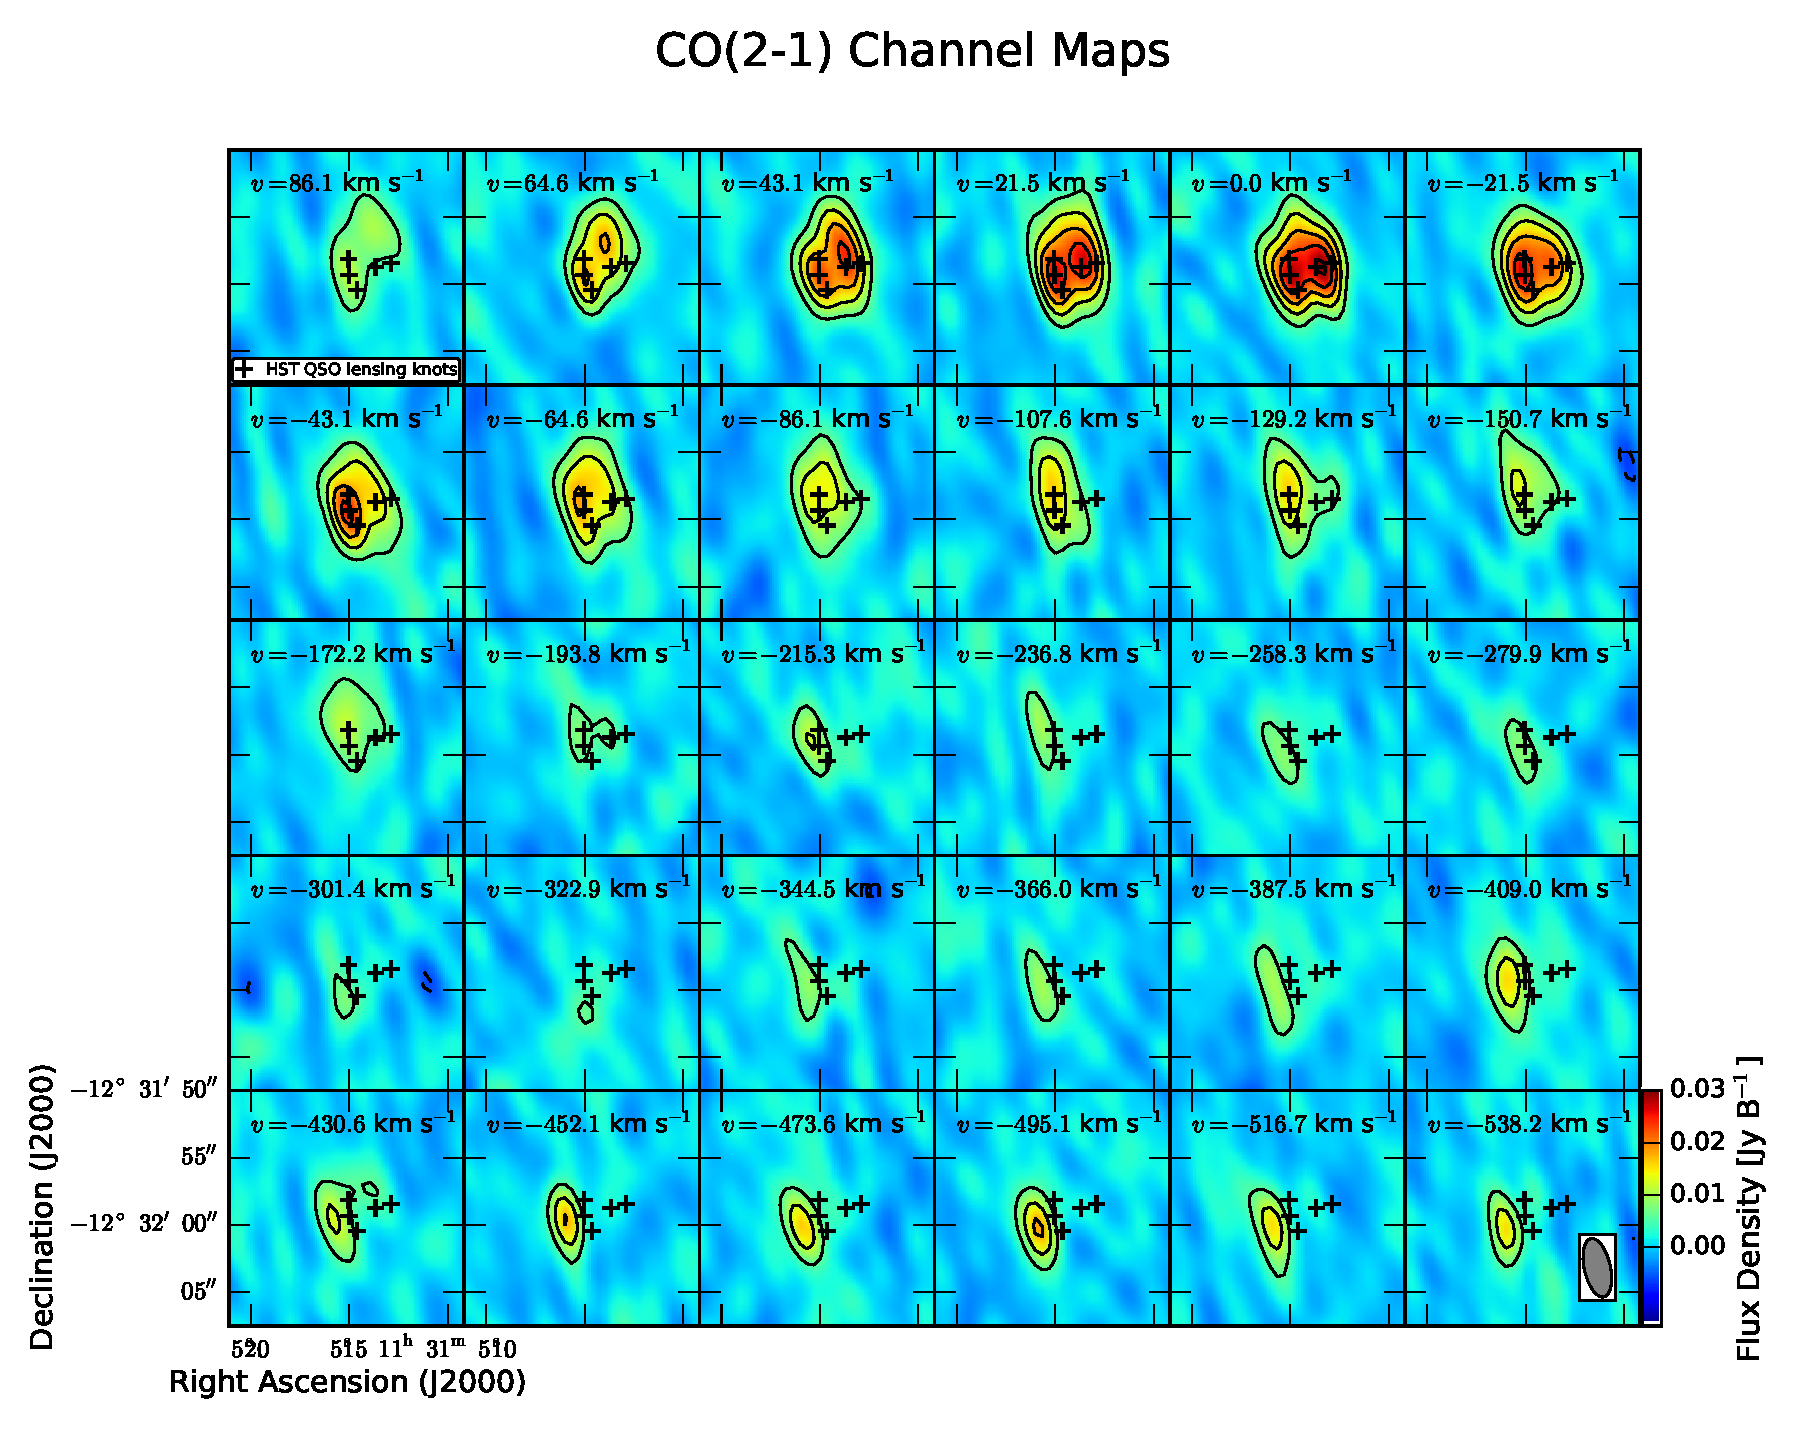
\includegraphics[width=\textwidth]{../Figures/co_channel_maps.eps}	 %
figures are in ../Figures/ for now, before we decided which ones will
definitely go into 
paper
\caption{
Black crosses indicate the position of the lensed AGN (components ABCD) and the
foreground lensing galaxy (component G) in the HST image.
 \label{fig:chanmap}}
\end{figure*}

\begin{figure*}[tbph]
\centering
\includegraphics[width=\textwidth]{../Figures/spatialSpec_offsetShifted.eps}   
   % figures are in ../Figures/ for now, before we decided which ones will
definitely go 
into paper
\caption{ 
Spatial spectra, binned by 3 pixels in each direction (1\farcs5)
 \label{fig:spatialSpec}}
\end{figure*}



\section{Continuum}


\begin{figure*}[tbph]
\centering
\includegraphics[width=0.8\textwidth]{../Figures/ContCO21.eps}	  
\caption{CO 21 moment0 with coninuum
 \label{fig:}}
\end{figure*}

\begin{figure*}[tbph]
\centering
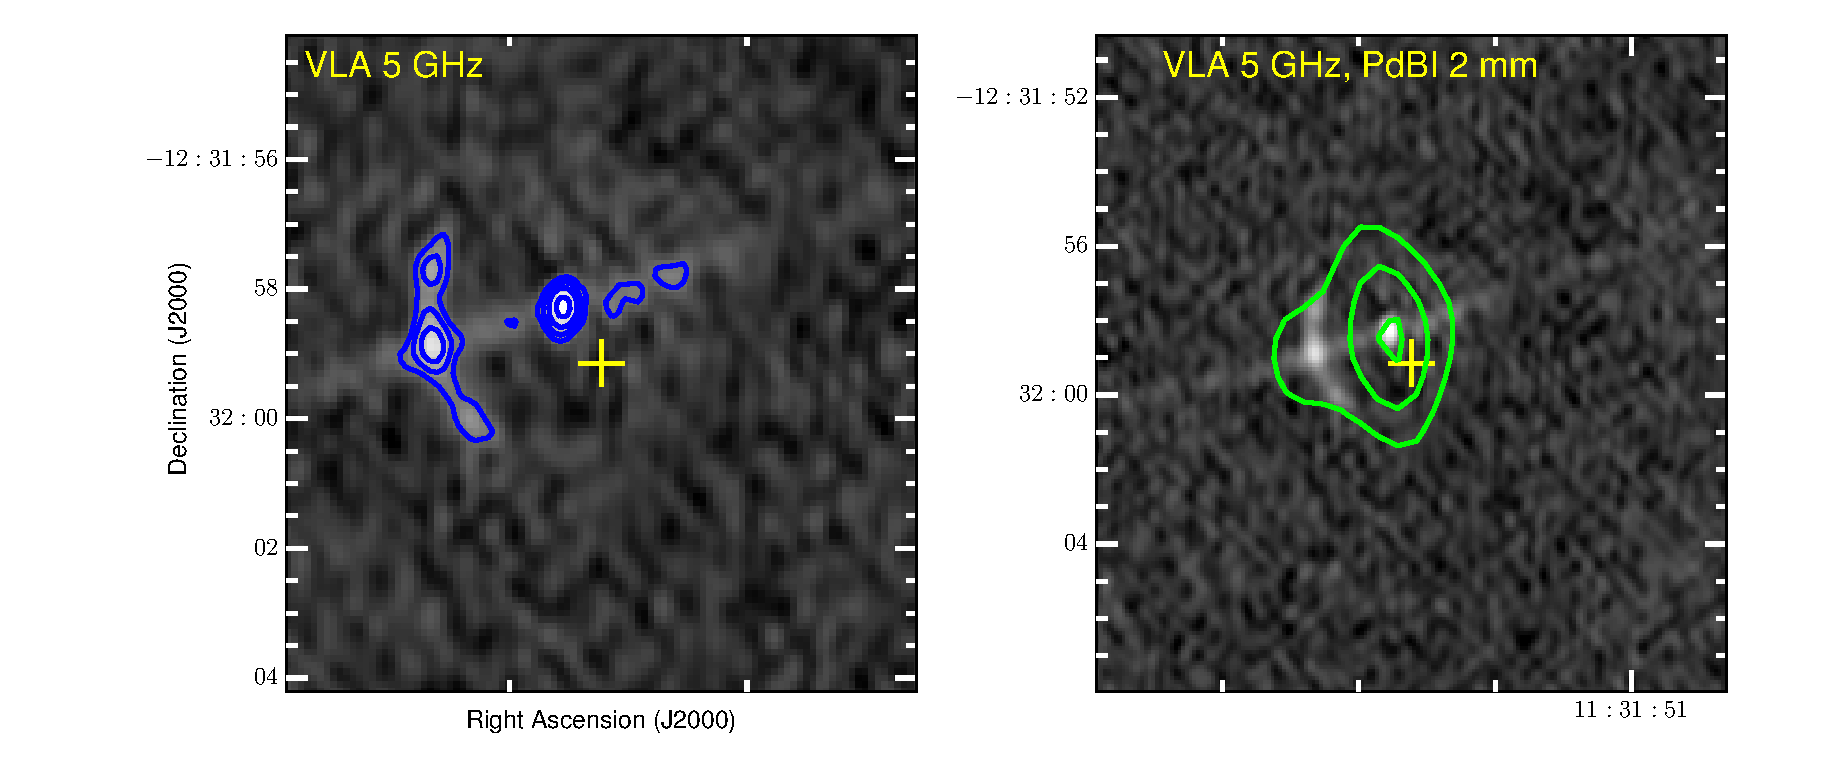
\includegraphics[width=0.8\textwidth]{../Figures/Cont2mm_5GHz_double.eps}    
\caption{VLA 5GHz continuum and PdBI 2mm continuum
 \label{fig:}}
\end{figure*}


\begin{figure*}[tbph]
\centering
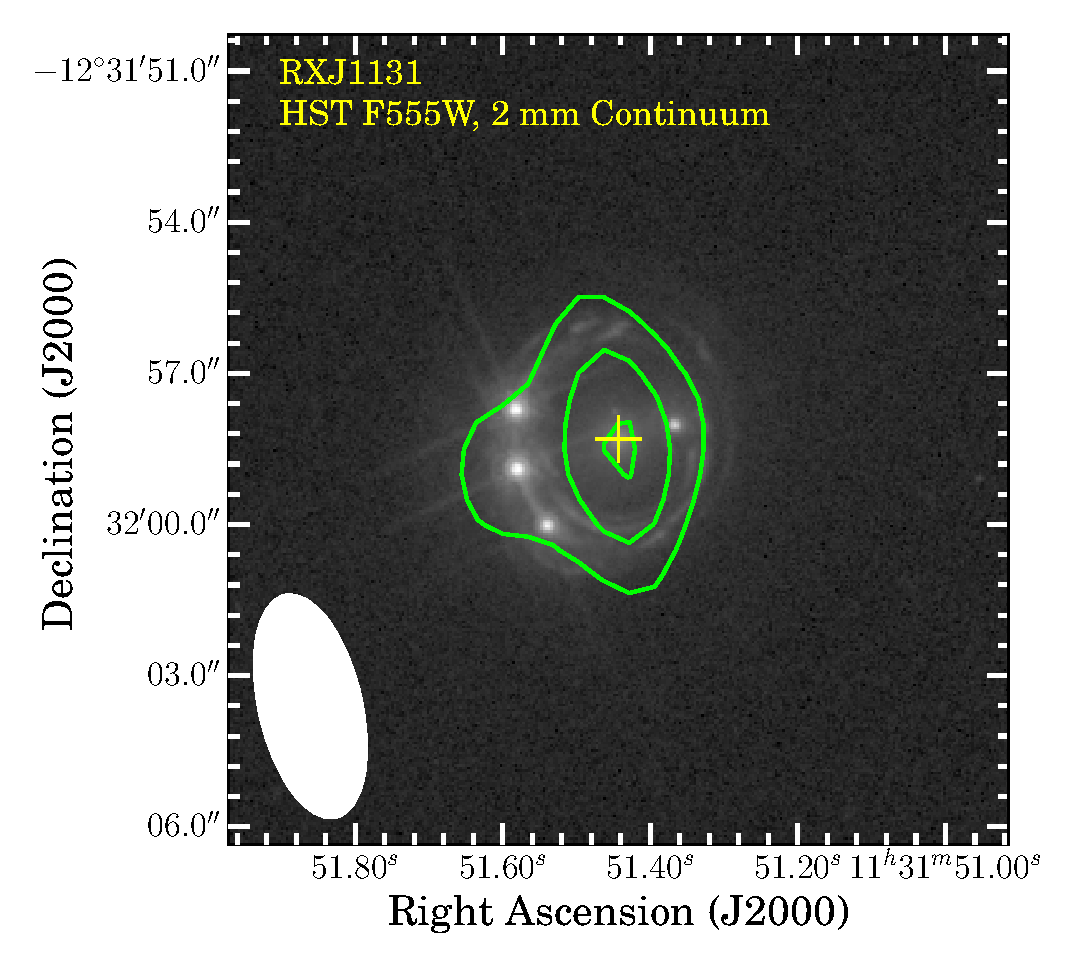
\includegraphics[width=0.35\textwidth]{../Figures/F555W_ContPdBI.eps}
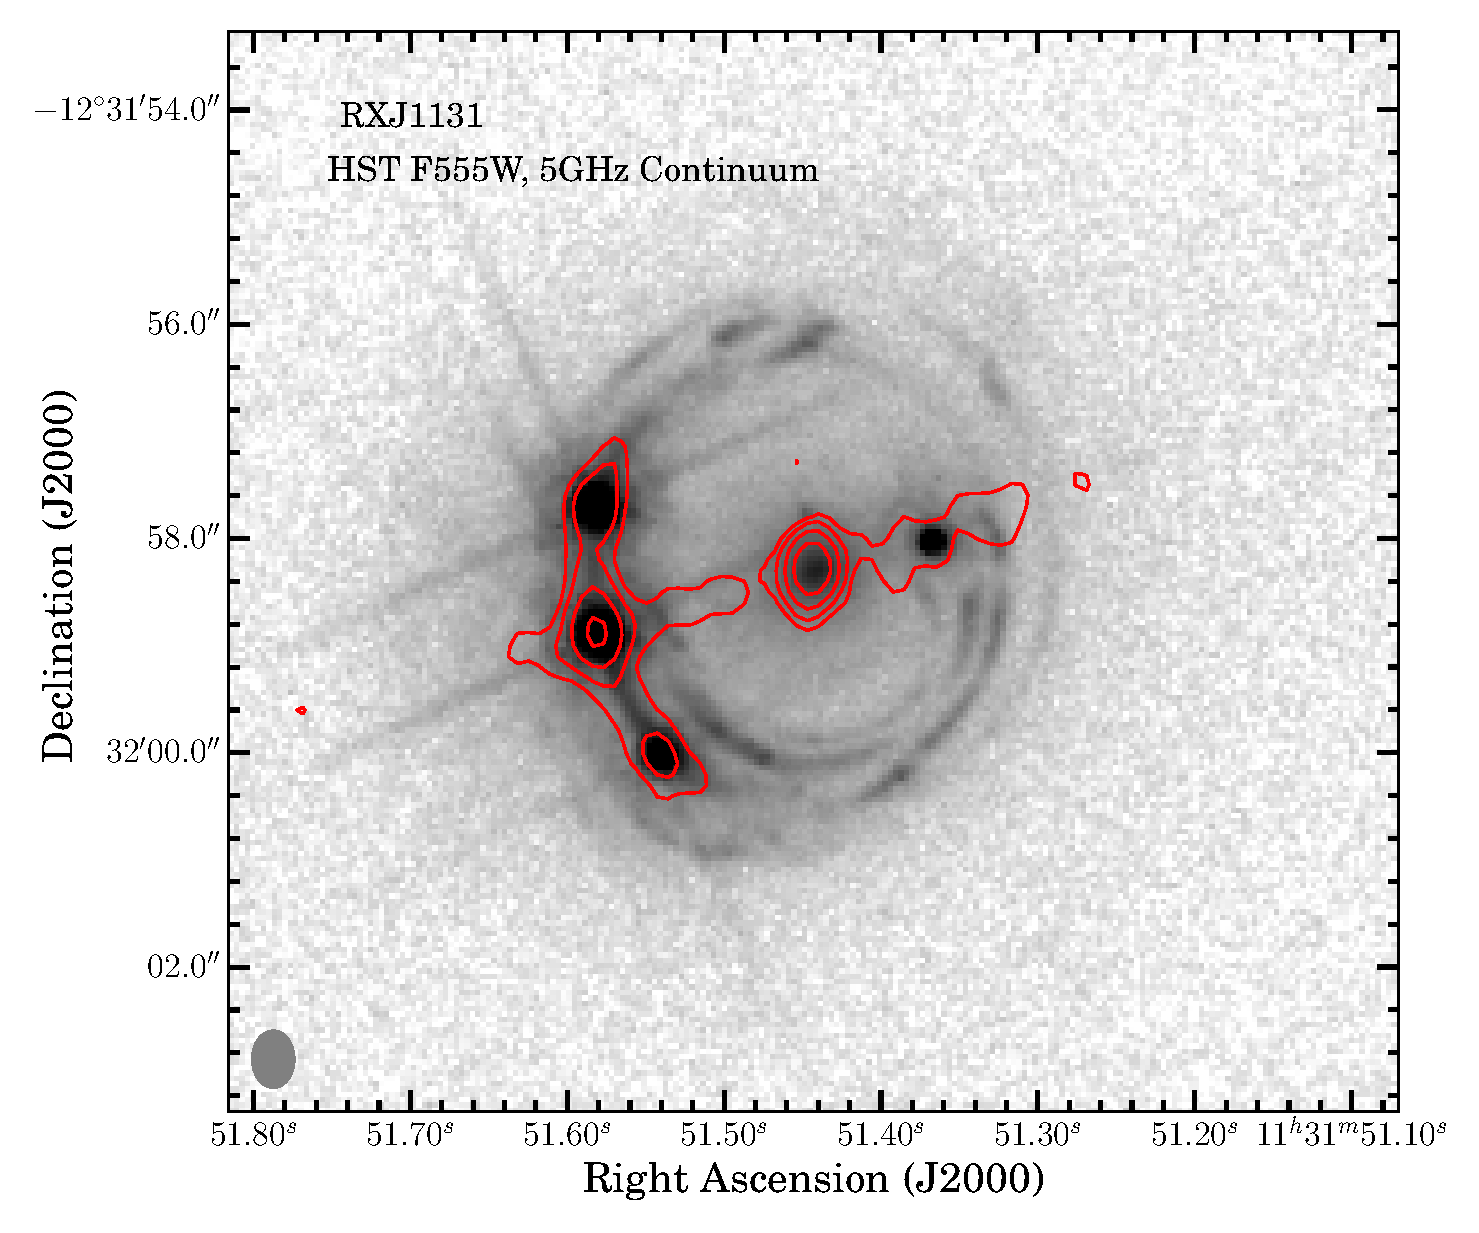
\includegraphics[width=0.55\textwidth]{../Figures/F555W_ContVLA.eps}
\caption{
radio continuum contours on HST image
 \label{fig:}}
\end{figure*}


%%%%%%%%%%%%%%%%%%%%%%%%%%%%%%%%%%%%%%%%%%
\section{SED}
\begin{figure*}[tbph]
\centering
\includegraphics[width=0.8\textwidth]{../Figures/FullSED.eps}	 
\caption{VLA 5GHz continuum and PdBI 2mm continuum
 \label{fig:}}
\end{figure*}

\begin{deluxetable}{lccc}[!htbp]
\centering
\tabletypesize{\scriptsize}
\tablecolumns{4}
\tablecaption{Photometry data}
\tablehead{\colhead{Wavelength} & \colhead{Frequency} & \colhead{Flux Density} & \colhead{Instrument}\\
\colhead{($\micron$)} & \colhead{(GHz)} & \colhead{(mJy)} & \colhead{ } \vspace{0.05in}
\\  \cline{1-4} \vspace{-0.05in} \\
\multicolumn{4}{c}{Combined/Unresolved}
}
\startdata
1.25    & 239834  & 1.009 $\pm$ 0.09    & CTIO/J-Band \\
1.65    & 181692  & 1.448 $\pm$ 0.12    & CTIO/H-Band \\
2.17    & 138153  & 2.064 $\pm$ 0.16    & CTIO/Ks-Band \\
3.4     & 88174.2 & 7.027 $\pm$ 0.14    & {\it WISE}/W1 \\
3.6     & 83275.7 & 5.618 $\pm$ 0.0021  & {\em Spitzer}/IRAC \\
4.5     & 66620.5 & 7.803 $\pm$ 0.0021  & {\em Spitzer}/IRAC \\
4.6     & 65172.3 & 8.872 $\pm$ 0.16    & {\it WISE}/W2 \\
5.8     & 51688.4 & 10.720 $\pm$ 0.0051 & {\it Spitzer}/IRAC \\
8.0     & 37474.1 & 14.470 $\pm$ 0.0041 & {\it Spitzer}/IRAC \\
12      & 24982.7 & 21.960 $\pm$ 0.42   & {\it WISE}/W3 \\
12      & 24982.7 & $<$400              & {\it IRAS} \\
22      & 13626.9 & 55.110 $\pm$ 1.9    & {\it WISE}/W4 \\
24      & 12491.4 & 70.204 $\pm$ 0.026  & {\it Spitzer}/MIPS \\
25      & 11991.7 & $<$ 500             & {\it IRAS} \\
60      & 4996.54 & $<$ 600             & {\it IRAS} \\
100     & 2997.92 & $<$ 1000            & {\it IRAS} \\
250     & 1199.17 & 289.4 $\pm$ 9.6     & {\it Herschel}/SPIRE \\
350     & 856.55  & 168.2 $\pm$ 8.6     & {\it Herschel}/SPIRE \\
500     & 599.585 & 56.8 $\pm$ 8.8      & {\it Herschel}/SPIRE \\
1387.93 & 216     & $<$2.492            & CARMA \\
2152.82 & 139.256 & 1.230 $\pm$ 0.220   & PdBI \\
\cutinhead{Foreground Lensing Galaxy (deblended bands)} \\ [-1.5ex]
0.555   & 540167  & 0.056 $\pm$ 0.006   & {\it HST}-ACS/V-Band \\
0.814   & 368295  & 0.238 $\pm$ 0.013   & {\it HST}-ACS/I-Band \\
1.6     & 187370  & 0.539 $\pm$ 0.041   & {\it HST}-NICMOS(NIC2)/H-Band \\
3.6     & 83275.7 & 0.585 $\pm$ 0.003\tna   & {\em Spitzer}/IRAC \\
4.5     & 66620.5 & 1.794 $\pm$ 0.0027\tna  & {\em Spitzer}/IRAC \\
5.8     & 51688.4 & 3.163 $\pm$ 0.0059\tna  & {\it Spitzer}/IRAC \\
8.0     & 37474.1 & 4.589 $\pm$ 0.0057\tna  & {\it Spitzer}/IRAC \\
2152.82 & 139.256 & 0.799 $\pm$ 0.082   & PdBI \\
61414   & 4.8815  & 0.866 $\pm$ 0.027   & VLA \\
\cutinhead{Background Galaxy RXJ1131 (deblended bands)}
0.555   & 540167  & 0.009 $\pm$ 0.0041\tnb  & {\it HST}-ACS/V-Band \\
0.814   & 368295  & 0.041 $\pm$ 0.0054\tnb  & {\it HST}-ACS/I-Band \\
1.6     & 187370  & 0.133 $\pm$ 0.004\tnb   & {\it HST}-NICMOS(NIC2)/H-Band \\
3.6     & 83275.7 & 5.034 $\pm$ 0.0021  & {\em Spitzer}/IRAC \\
4.5     & 66620.5 & 6.009 $\pm$ 0.0017  & {\em Spitzer}/IRAC \\
5.8     & 51688.4 & 7.557 $\pm$ 0.003   & {\it Spitzer}/IRAC \\
8.0     & 37474.1 & 9.881 $\pm$ 0.0039  & {\it Spitzer}/IRAC\\
2152.82 & 139.256 & 0.400 $\pm$ 0.082\tnc   & PdBI \\
61414   & 4.8815  & 1.273 $\pm$ 0.042   & VLA
\enddata
\label{tab:photometry}
\tablecomments{The IRAC photometry for channel 1 (3.6\,$\micron$) is extracted directly from the image and
from the Spitzer Heritage Archive for channels 2$-$4 (4.5, 5.8, and 8.0\,$\micron$). All upper limits are 3$\sigma$.}
\tablenotetext{a}{Flux obtained using aperture photometry after subtracting the emission of RXJ1131 from the total emission.}
\tablenotetext{b}{A contribution from the quasar has been removed (see C06), and thus the flux density corresponds to the host galaxy only.}
\tablenotetext{c}{Flux extracted from the residual map after subtracting a point-source model.}
\tablerefs{The {\it HST} photometry is adopted from C06.}
\end{deluxetable}






%%%%%%%%%%%%%%%
\end{document}